%!TEX root = ../Project.tex

\subsection{Database structure}
\label{developmentdatabasestructure}

As relational databases are so popular and are supported in many software
frameworks, there is no advantage to choosing a database model other than
relational. Web frameworks abstract away any code related to a specific
database product using an \gls{orm}, so the module allocation application can
be written without regard for the final database product that \gls{itservices}
will use to deploy the application.

Preliminary conversations with departmental administrators informed the
database structure, and in fact provided answers to the questions outlined in
Section~\ref{sec:researchdatabase}. Firstly, there are several entities stored
by the University that will be useful to this system, which have the
properties given in Table~\ref{development_database_uni_entities}. Each module
is given a number of credits representing the estimated workload for that
module, and each student must take 120 credits every academic year.

\begin{table}
  \begin{center}
    \begin{tabular}{ | l | l | }
      \hline
      \textbf{Entity} & \textbf{Properties} \\
      \hline
      Student    & Username (unique), \gls{routecode}, \gls{stage} \\
      Module     & Module code (unique), module name, number of credits, maximum class size \\
      \hline
    \end{tabular}    
  \end{center}
  \caption{Entities and their properties as stored by the University of York}
  \label{development_database_uni_entities}
\end{table}

The two pilot departments currently use paper forms, some of which are given
in Appendix~\ref{sec:paperforms}. In order to create a scalable system that
could be used across any number of departments, I first generalised the paper
forms provided by the pilot departments. This generalisation involved the
following observations:

\begin{itemize}
  \item Each degree type (single subject, joint honours, etc) can receive a different form
  \item Each form contains one or more groups, and each group contains one or more modules
  \item A student will be allocated a certain number of modules from each group
\end{itemize}

These observations led to the creation of a database structure given in
Table~\ref{development_database_schema}.

\begin{table}
  \begin{center}
    \begin{tabular}{ | l | l | }
      \hline
      \textbf{Entity} & \textbf{Properties} \\
      \hline
      Sheet & \underline{\gls{routecode}}, \underline{\gls{stage}}, student help \\
      Group & \emph{Sheet}, title, student help, credits to allocate \\
      Module & \underline{module code}, module name, \emph{Department} \\
      Module Availability & \emph{Module}, credits, student min, student cap \\
      Student & \underline{username}, date ranked, \emph{Sheet}, \emph{Department} \\
      Elective & \emph{Student}, \emph{Group}, credits \\
      Department & name \\
      Staff & \underline{username}, \emph{Department} \\
      Allocation & \emph{Student}, \emph{Module Availability} \\
      Choice & \emph{Student}, \emph{Module Availability}, rank \\
      \hline
    \end{tabular}
  \end{center}
  \caption{Entities stored in the application (\underline{primary key}
    underlined (automatically incrementing integer if none given), \emph{foreign
    key} in italics)}
  \label{development_database_schema}
\end{table}

As one would expect from its name, a sheet entity is a replacement for the
current paper sheets used by departments. It is unique by type of student
(\gls{routecode}) and by their year of study. A sheet can contain one or more
group entities. There is a many-to-many relationship between groups and module
availabilities. A module availability is an instance of a module in a specific
term or year. We use a module availability entity as this is sometimes used by
the University when a module must be run twice in one year to account for it
being a popular choice among students. In that case, the module would have the
same module code but might have a different class size.

Every student is assigned to a specific sheet, which informs the groups and
modules that are available to them (in terms of functional dependencies, this
can be written $Student \rightarrow Sheet$, indicating that a student's degree
type and year of study determines which sheet they view). Every choice the
student makes is stored in the database along with the rank they gave that
module, and an allocation is simply a student, module pair.

\subsubsection{Entity-relationship diagram}

From Table~\ref{development_database_schema} and Figure~\ref{er_diagram} (an
\gls{er} diagram for the module allocation system), one can use the tests
given in Table 10.1 of \emph{Fundamentals of Database Systems}
\cite{ElmasriFundamentals_2004} to see that this database is in \gls{3nf}. It
is in \gls{1nf} as there are no non-single attributes or nested relations. It
is in \gls{2nf}; the only table with a composite primary key is Sheet, and the
`student help' attribute is dependent on the combination of \gls{routecode}
and \gls{stage}, not on just one of them. Finally, it is in \gls{3nf} as there
is no transitive dependency of non-primary key attributes.

\begin{landscape}
  \begin{figure}
    \centering
    \fbox{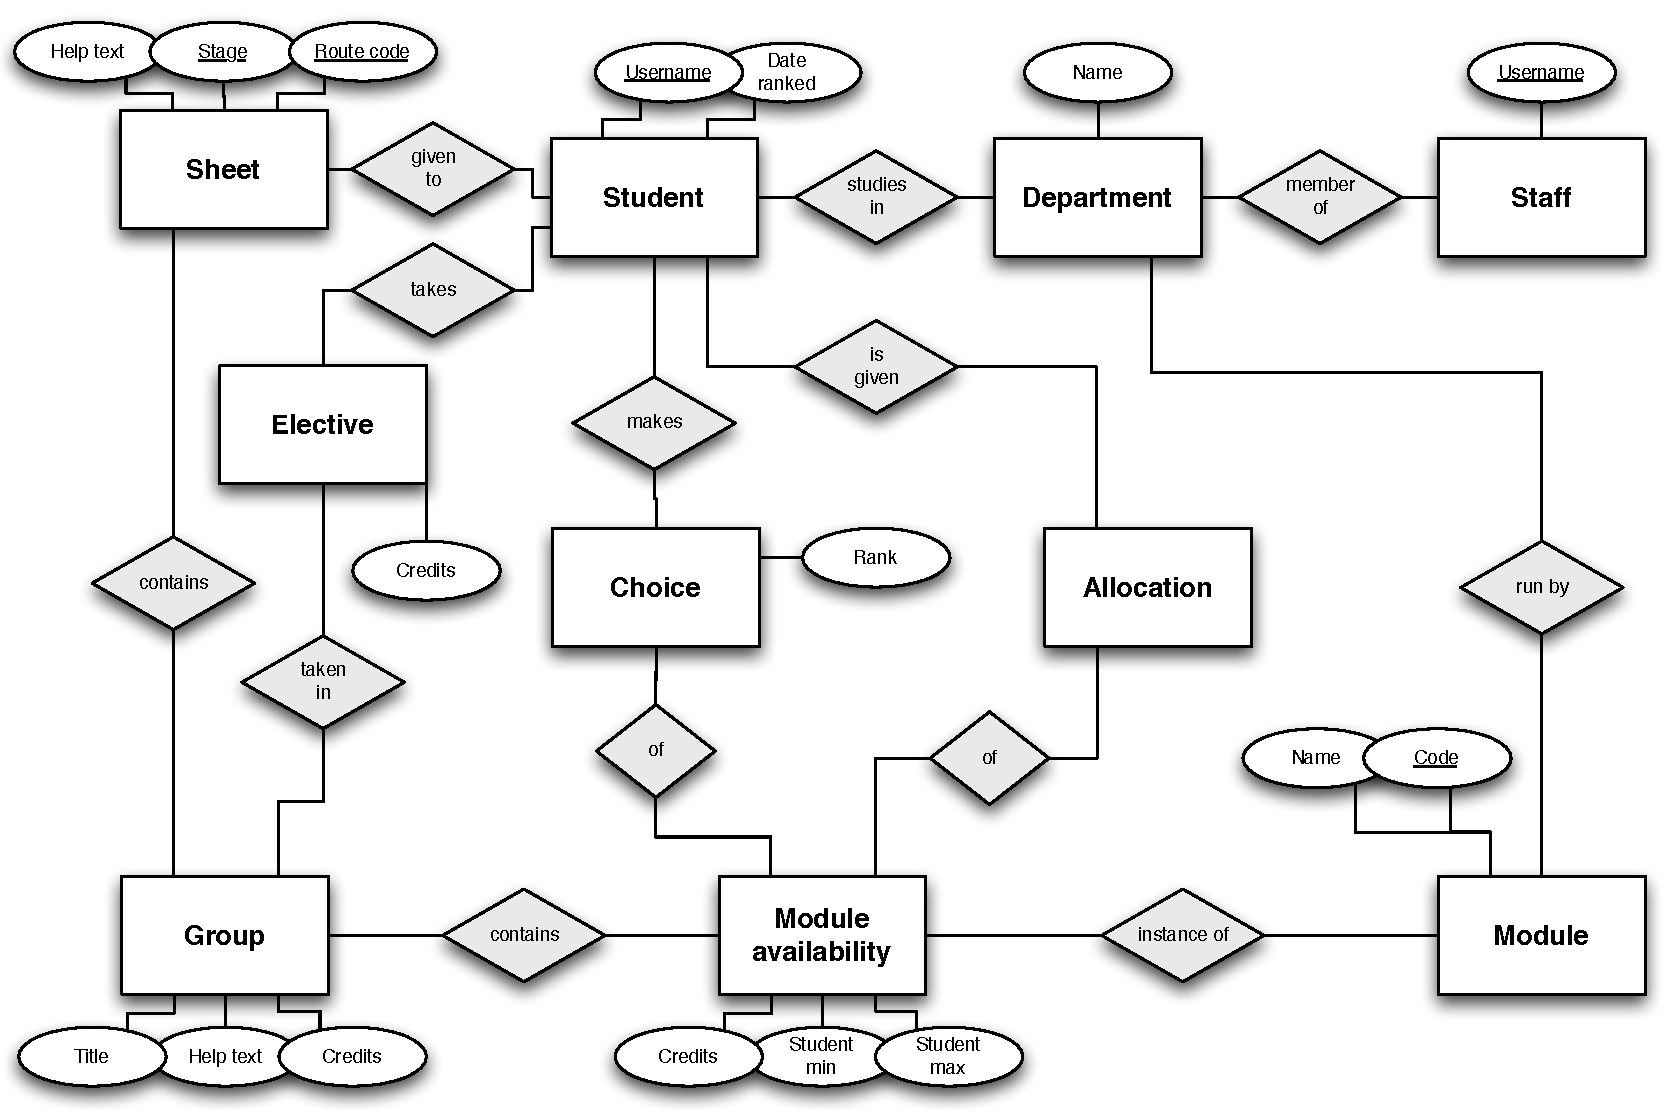
\includegraphics[width=0.9\linewidth]{inc/er_diagram.pdf}}
    \caption{Entity-relationship diagram for the module allocation system}
    \label{er_diagram}
  \end{figure}
\end{landscape}
